\documentclass[a4paper,11pt]{ctexart}
\usepackage{amssymb}
\usepackage{amsmath}

\usepackage{graphicx}
\usepackage{geometry}
\geometry{top=2.5cm, bottom=1.8cm, left=2cm, right=2.5cm}
\usepackage{booktabs}
\usepackage{float}

%================ 行距 ================
\usepackage{setspace}
\setstretch{1.3}

\usepackage{calc}
\setlength{\lineskip}{\baselineskip-\ccwd}
\setlength{\lineskiplimit}{2.5pt}

\usepackage{enumitem}
\usepackage{listings}
\lstset{
    basicstyle          =   \sffamily,          % 基本代码风格
    keywordstyle        =   \bfseries,          % 关键字风格
    commentstyle        =   \rmfamily\itshape,  % 注释的风格，斜体
    stringstyle         =   \ttfamily,  % 字符串风格
    flexiblecolumns,                % 别问为什么，加上这个
    numbers             =   left,   % 行号的位置在左边
    showspaces          =   false,  % 是否显示空格，显示了有点乱，所以不现实了
    numberstyle         =   \zihao{-5}\ttfamily,    % 行号的样式，小五号，tt等宽字体
    showstringspaces    =   false,
    captionpos          =   t,      % 这段代码的名字所呈现的位置，t指的是top上面
    frame               =   lrtb,   % 显示边框
}

\renewcommand{\d}{\mathop{}\!\mathrm{d}}
\everymath{\displaystyle}


\begin{document}

\title{微分方程数值解大作业1}
\author{庞逸天 523070910095}
\maketitle

\section{Task 1}
所使用的四个核心算法的matlab代码记为pdf提供的代码，未做修改，在此不做展示.\par
在任务1中，选择的函数为$u(x,y)=x(x-1)y(y-1)$，使用的matlab代码为：
\begin{lstlisting}[language=Matlab]
%task1
%8-512的网格数按对数均匀分布
N_list = unique(round(logspace(log10(8), log10(512), 31)));
num = length(N_list);

%初始化时间矩阵与误差矩阵
times = NaN(num, 4); 
errors = zeros(num, 1);

fprintf(' N \t\t DST(s) \t BlockLU(s) \t Jacobi(s) \t GS(s)\n');
for k = 1:length(N_list)
    N = N_list(k);
    
    %DST
    tic; U_dst = DSTPS(N); times(k,1) = toc;
    
    %BlockLU
    tic; U_lu = BlockLU(N); times(k,2) = toc;
    
    %Jacobi
    if N <= 128
        tic; U_jacobi = PSJacobi(N); times(k,3) = toc;
    else
        times(k,3) = NaN; 
    end
    
    %Gauss-Seidel
    if N <= 128
        tic; U_gs = PSGS(N); times(k,4) = toc;
    else
        times(k,4) = NaN;
    end
    
    %计算精确解与误差
    h = 1/N;
    x = h*(1:N-1);
    [X, Y] = meshgrid(x, x);
    U_exact = X.*(X-1).*Y.*(Y-1);
    errors(k) = max(max(abs(U_dst - U_exact)));
    fprintf(N, times(k,1), times(k,2), times(k,3), times(k,4));
end

%绘制时间图
figure('Position', [100, 100, 700, 500]);
plot(N_list, times(:,1), '-ro', 'LineWidth', 2, 'MarkerSize', 6); hold on;
plot(N_list, times(:,2), '-bs', 'LineWidth', 2, 'MarkerSize', 6);
plot(N_list, times(:,3), '-g^', 'LineWidth', 2, 'MarkerSize', 6);
plot(N_list, times(:,4), '-md', 'LineWidth', 2, 'MarkerSize', 6);

set(gca, 'XScale', 'log', 'YScale', 'log');
xticks(N_list);
xticklabels(string(N_list));
grid on;

xlabel('网格数N(对数均分)', 'FontSize', 12, 'FontWeight', 'bold');
ylabel('计算耗时/秒 (对数均分)', 'FontSize', 12, 'FontWeight', 'bold');
title('Poisson方程不同求解算法的耗时', 'FontSize', 14);
legend('DST', 'LU分解', 'Jacobi 代', 'Gauss-Seidel迭代', ...
       'Location', 'northwest', 'FontSize', 11);

%绘制网格数为256数值解与精确解误差图
figure;
surf(X, Y, abs(U_dst - U_exact));
title(['N = ', num2str(N), ' 时 DST的误差']);
xlabel('x'); ylabel('y'); zlabel('Error');
colormap('jet'); colorbar;
\end{lstlisting}

第一部分是对数据的初始化，选择了从8-512中按对数均匀分布的32个不同的网格数.\par
第二部分分别使用四种算法在不同网格数下求解Poisson方程，并记录每种算法的计算时间.需要注意的是，由于两种迭代算法在较大网格数下计算时间过长，因此当网格数超过128时，直接将其时间记录为NaN(大网格数的结果会使用图表展示).\par
第三部分分别绘制了不同算法的计算时间随网格数变化的图表，以及当网格数为256时，DST算法的数值解与精确解的误差图.\par 
所得到的两张图片为：
\begin{figure}[htbp]
    \centering
    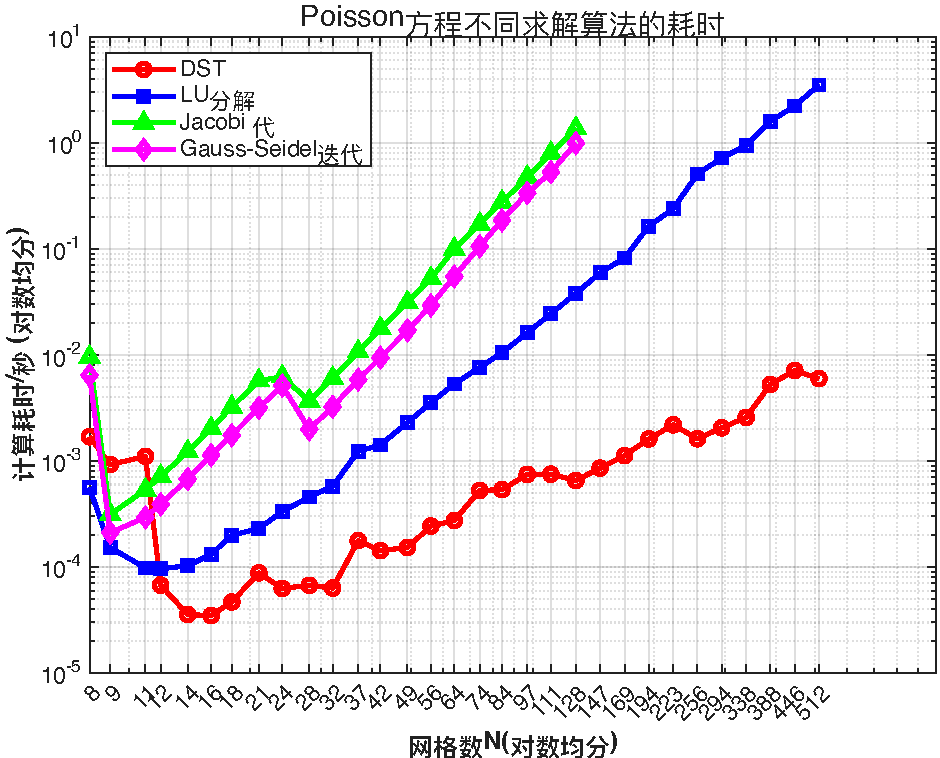
\includegraphics[width=0.8\textwidth]{algo_time.pdf}
\end{figure}
\begin{figure}[H]
    \centering
    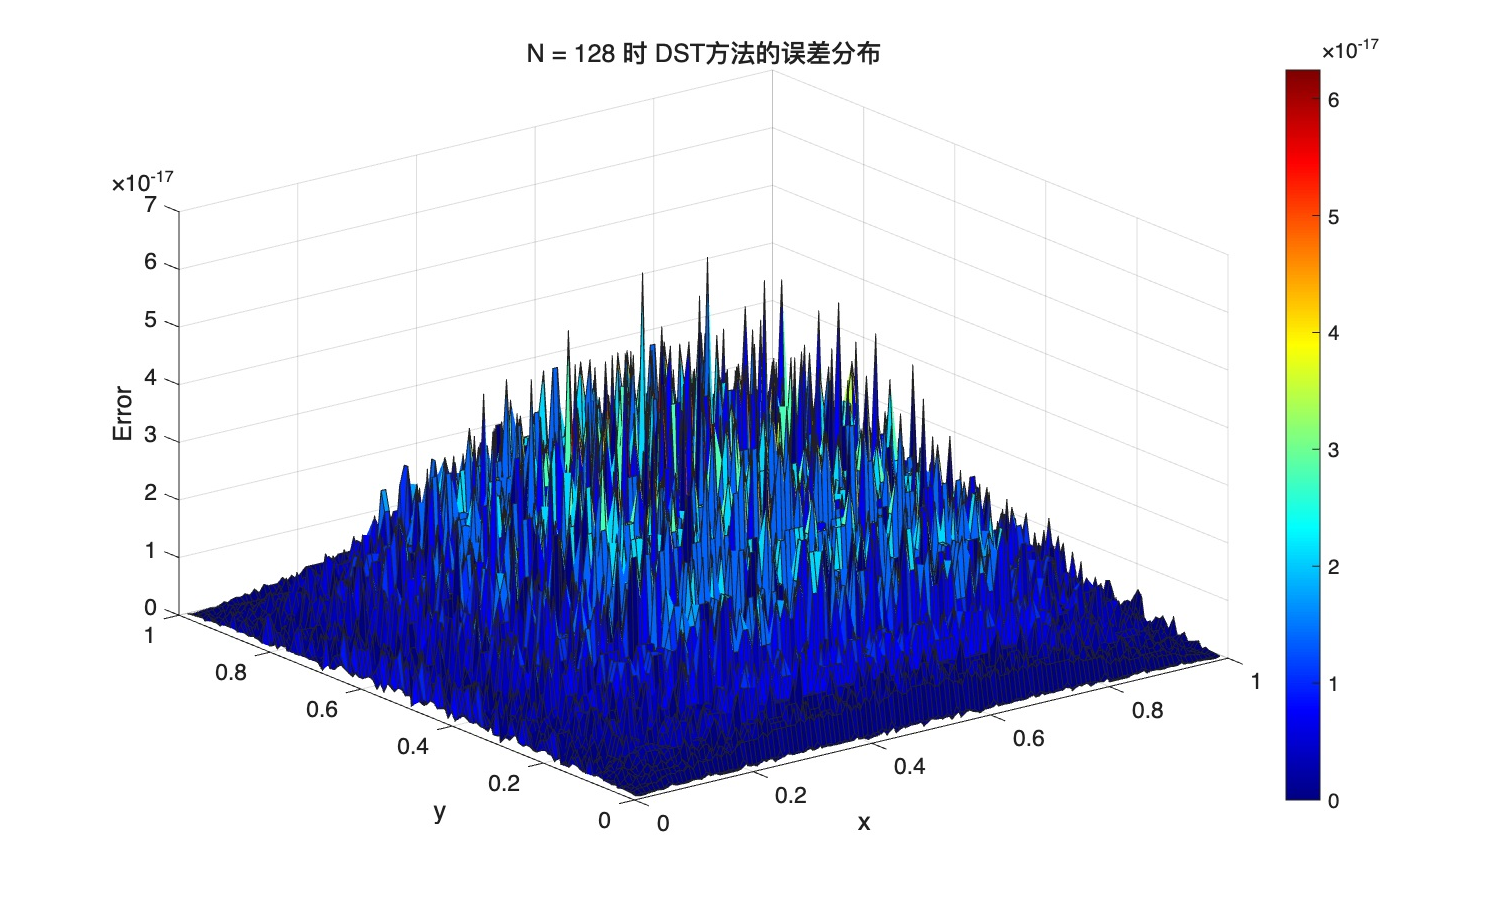
\includegraphics[width=0.9\textwidth]{dst_error.pdf}
\end{figure}
除此之外，为了强调迭代算法在大网格数下的计算时间过长，单独绘制了迭代算法的计算时间图表，结果如下：
\begin{table}[htbp]
    \centering
    \renewcommand{\arraystretch}{1.5}
    \begin{tabular}{ccccc}
        \toprule
        网格数 & DST(s) & LU分解(s) & Jacobi迭代(s) & Gauss-Seidel迭代(s) \\
        \midrule
        8 & 0.005294 & 0.001524 & 0.007225 & 0.009104 \\
        16 & 0.002533 & 0.000304 & 0.002134 & 0.001513 \\
        32 & 0.000170 & 0.000820 & 0.023972 & 0.007784 \\
        64 & 0.000456 & 0.005460 & 0.099198 & 0.054517 \\
        128 & 0.000890 & 0.039573 & 1.368376 & 0.991336 \\
        256 & 0.001941 & 0.556518 & 2.858811 & 15.815365 \\
        512 & 0.006481 & 4.081208 & 331.678322 & 262.940940 \\
        \bottomrule
    \end{tabular}
\end{table}
从图像和表格中可以观察到如下几点：
\begin{enumerate}[label=(\arabic*)]
    \item DST算法的计算时间远小于其他三种算法
    \item 两种迭代方法在较大网格数下的计算时间急剧增加
    \item DST的时间复杂度相较于其他三者更低
\end{enumerate}

\section{Task 2}

\subsection{理论分析}

对于边界条件为非齐次Dirichlet条件的二维Poisson方程$\begin{cases}
    \Delta u(x,y) = f(x,y), (x,y)\in \Omega\\
    u(x,y) = \alpha(x,y), (x,y)\in \partial\Omega
\end{cases}$，如果想要使用DST算法对其求解，首先需要将左侧的系数矩阵写成齐次情形时的样子.\par
考虑横纵坐标的网格数均为$N$，则$h=k=\frac{1}{N}$，那么五点差分格式可以写为：
\[\begin{cases}
\frac{u_{i+1,j}+u_{i-1,j}+u_{i,j+1}+u_{i,j-1}-4u_{i,j}}{h^2}=f_{i,j}, 1\leq i,j\leq N-1\\
u_{i,0}=\alpha_{i,0}, u_{i,N}=\alpha_{i,N}, u_{0,j}=\alpha_{0,j}, u_{N,j}=\alpha_{N,j}
\end{cases}\]
我们需要对其中包含边界值的项进行修正，使得其满足齐次情形的矩阵.\par
以$j=1$为例，有$u_{i+1,1}+u_{i-1,1}+u_{i,2}+u_{i,0}-4u_{i,1}=h^2 f_{i,1}$.\par
此处边界值$u_{i,0}=\alpha(x_i,0)$，希望作调整使得$u'_{i,0}=0$，则可以将这一项移到右侧
\[u_{i+1,1}+u_{i-1,1}+u_{i,2}+u'_{i,0}-4u_{i,1}=h^2 f_{i,1}+u_{i,0}\]
其中$u'_{i,0}=0$.\par
最后，在等式两边同除$h^2$，将形式还原
\[\frac{u_{i+1,1}+u_{i-1,1}+u_{i,2}+u'_{i,0}-4u_{i,1}}{h^2}=f_{i,1}+\frac{u_{i,0}}{h^2}\]
这样，我们可以将非齐次的边界引入到方程的右侧，此时左侧的系数矩阵就满足了齐次情形的形式，可以使用DST算法进行求解.\par
对于其他边界条件的处理方法与上述类似，都是将包含边界值的项移到方程的右侧，将边界值调整为0.

\subsection{算法实现}

对给出的dst代码稍作修改即可得到满足非齐次边界条件的DST算法，具体改动在于需要自行调整方程的右侧矩阵，而不是直接使用原来的$f$矩阵，最终的matlab代码如下：
\begin{lstlisting}[language=Matlab]
    %task2

%网格数及步长
N = 256; 
h = 1/N;
x = h*(1:N-1); 
y = h*(1:N-1);
[X, Y] = meshgrid(x,y);

%初始的右侧矩阵
F = -4*ones(N-1,N-1);

%边界处的精确解 
u_bottom = x.^2;             
u_top = x.^2+1;         
u_left = y.^2;             
u_right = 1+y.^2;         

%为了使左侧矩阵形如齐次情形，将右侧矩阵在临近边界处做调整
F(1,:) = F(1,:)+u_bottom / h^2;
F(end,:) = F(end,:)+u_top / h^2;
F(:,1) = F(:,1)+u_left' / h^2;
F(:,end) = F(:,end)+u_right' / h^2;

%使用快速 DST 求解
lambda = 4*sin(pi*x/2).^2;
T = dst(dst(F)')';
V = zeros(N-1);
for i = 1:N-1
    for j = 1:N-1
        V(i,j) = T(i,j)/(lambda(i)+lambda(j));
    end
end
V = 4*h^4*V;
U_num = dst(dst(V)')';

%绘图计算误差
U_exact = X.^2+Y.^2;

figure;
surf(X, Y, abs(U_num - U_exact)),shading interp;
title(['N = ', num2str(N), ' 时 DST的误差']);
xlabel('x'); ylabel('y'); zlabel('Error');
colormap('jet'); colorbar;
\end{lstlisting}
所得到的误差图为：
\begin{figure}[htbp]
    \centering
    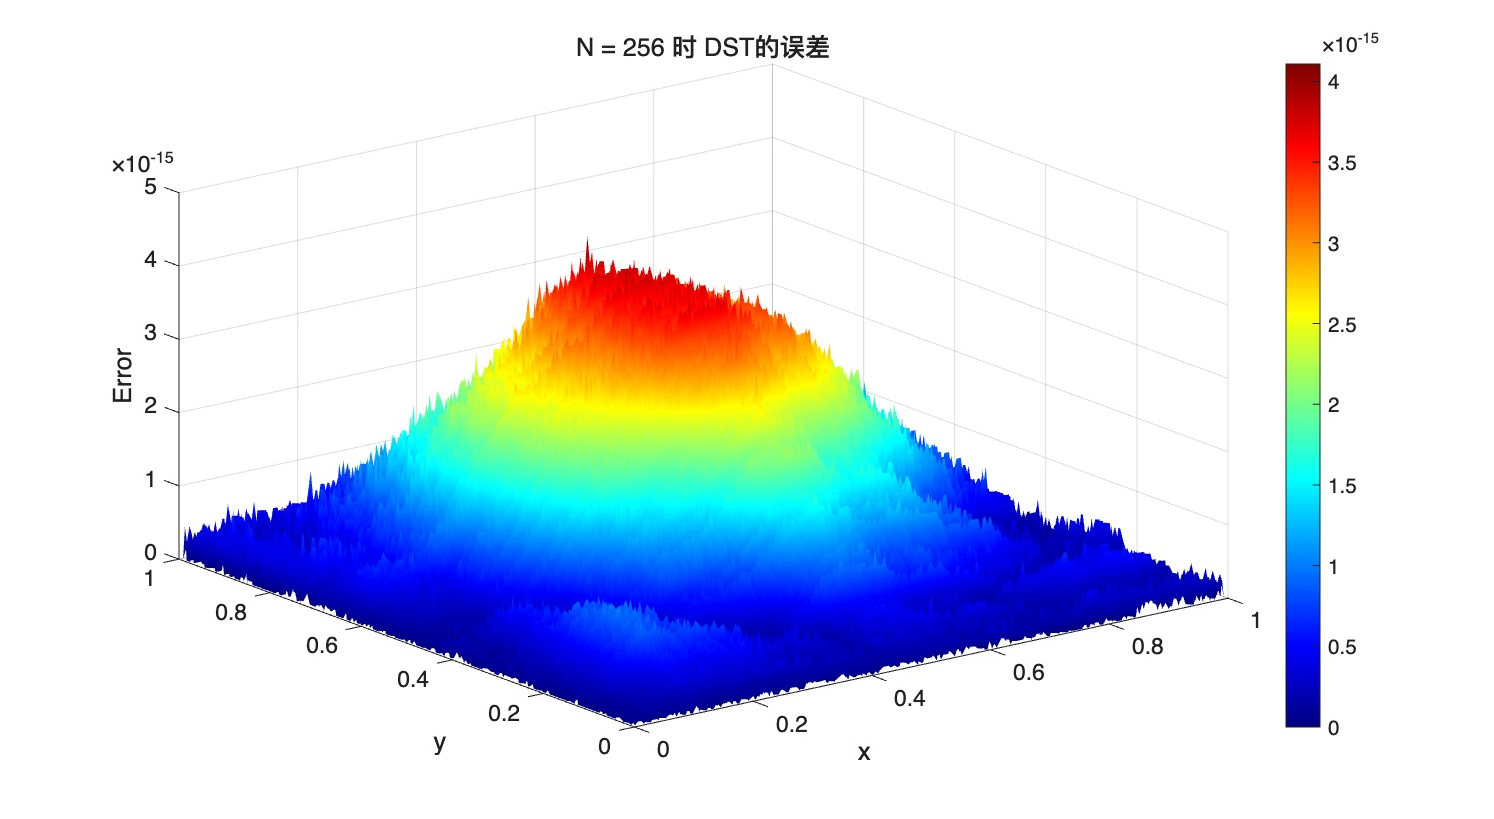
\includegraphics[width=0.9\textwidth]{dst_error2.pdf}
\end{figure}

\section{task 3}
\subsection{理论分析}
当边界从$(0,1)\times(0,1)$变为$(0,a)\times(0,b)$，且网格数不一定相等后，源代码中$A,B$两个矩阵对应的特征向量相等的特性不再成立，因此我们需要对$A,B$两个矩阵分别计算其特征向量，然后使用dst进行求解.

\subsubsection{算法实现}

\begin{lstlisting}[language=Matlab]
%task 3

% 设置区域和网格
a = 2; 
b = 1;
Nx = 128;
Ny = 256;
h = a/Nx;
k = b/Ny;

x = h*(1:Nx-1);
y = k*(1:Ny-1);
[X, Y]=meshgrid(x,y);

U_exact = X.*(X-2).*Y.*(Y-1);
F = -2*(X.^2-2*X+Y.^2-Y);

%计算 X 和 Y 方向的特征值
lambda_y = (4/k^2)*sin(pi*(1:Ny-1)/(2*Ny)).^2;
lambda_x = (4/h^2)*sin(pi*(1:Nx-1)/(2*Nx)).^2;


T = dst(dst(F)')'; 
V = zeros(Ny-1, Nx-1);

for i = 1:Ny-1
    for j = 1:Nx-1
        V(i,j) = T(i,j) / (lambda_y(i) + lambda_x(j));
    end
end

V = 4/(Nx*Ny)*V;
U_num = dst(dst(V)')';

%计算误差与绘图
figure;
surf(X, Y, abs(U_num - U_exact)),shading interp; 
title('一般矩形区域上的误差分布');
xlabel('x'); ylabel('y'); zlabel('Error');
shading interp; colormap('jet'); colorbar;
\end{lstlisting}

最终得到的误差图为：
\begin{figure}[H]
    \centering
    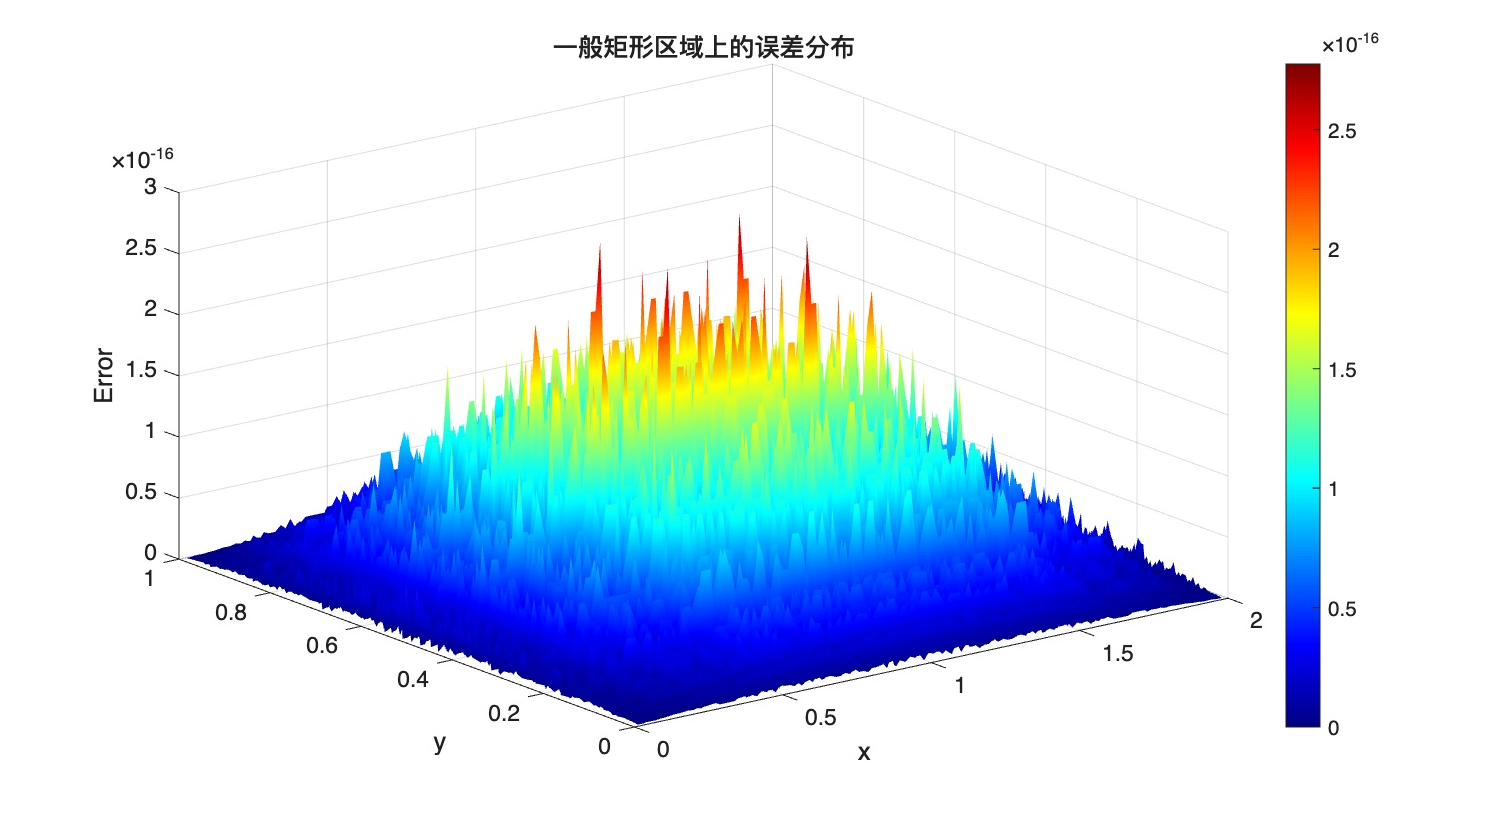
\includegraphics[width=0.9\textwidth]{dst_error3.pdf}
\end{figure}

\end{document}
